\chapter{Fourier Analysis and Sampling}
\label{chapter:FourierAnalysisSampling}

\index{Fourier analysis}
\textbf{Fourier analysis} refers to a collection of tools that can be applied to express a function in terms of complex sinusoids, called basis elements, of different frequencies.
The result of the decomposition is the amplitude and the phase to be imparted to each basis element in the reconstruction.
This decomposition is termed the \defn{Fourier analysis}{frequency domain} representation of the original signal.

Fourier analysis is extremely useful in engineering, with a myriad of applications.
Part of its appeal lies in the fact that basis elements are characteristic functions of linear time-invariant systems.
This property, which may seem nebulous at this point, is instrumental in solving many challenging problems, and makes Fourier analysis a powerful methodology for the design of communication systems.
We assume that the reader is familiar with basic Fourier analysis, and only review details that are pertinent to our treatment of communication systems.
This is not intended to be a comprehensive treatment of the subject.


\section{Fourier Series}
\label{section:FourierSeries}

Fourier series can be employed to express, as weighted sums of sinusoidal components, either periodic functions or functions that are time-limited.
Suppose that the signal $s(t)$ is zero for all $|t|\geq\frac{T}{2}$, is integrable and satisfies
\begin{equation*}
%\| s(t) \|^2 \triangleq
\int_{\mathbb{R}} |s(t)|^2 dt =
\int_{-\frac{T}{2}}^{\frac{T}{2}} |s(t)|^2 dt < \infty .
\end{equation*}
Then, $s(t)$ possesses a \defn{Fourier analysis}{Fourier series} representation, which is defined by
\begin{equation} \label{equation:FourierSeries1}
s(t) = \begin{cases} \sum_{k=-\infty}^{\infty}
\hat{s}_k e^{2 \pi i \frac{k}{T} t}, & \mathrm{if} \; |t| \leq \frac{T}{2} \\
0, & \text{otherwise} \end{cases}
\end{equation}
where the Fourier series coefficients $\{ \hat{s}_k : k \in \mathbb{Z} \}$ are given by
\begin{equation*}
\hat{s}_k = \frac{1}{T} \int_{-\frac{T}{2}}^{\frac{T}{2}}
s(t) e^{-2 \pi i \frac{k}{T} t} dt .
\end{equation*}
We can use the standard rectangular function $\mathrm{rect}(\cdot)$, defined by
\begin{equation} \label{equation:RectangularFunction}
\mathrm{rect} (t) = \begin{cases} 1, & \mathrm{if}\; |t| < 0.5 \\
0, & \text{otherwise} \end{cases}
\end{equation}
to simplify \eqref{equation:FourierSeries1}, and rewrite the Fourier representation of $s(t)$ as
\begin{equation} \label{equation:FourierSeries2}
s(t) = \sum_{k=-\infty}^{\infty}
\hat{s}_k e^{2 \pi i \frac{k}{T} t}
\mathrm{rect} \left( \frac{t}{T} \right) .
\end{equation}
If $s(t)$ is periodic with $s(t+T)=s(t)$, instead of being zero for $|t|>\frac{T}{2}$, then the same result holds without the rectangular window function.

From a vector space perspective, \eqref{equation:FourierSeries2} asserts that $s(t)$ can be expressed as a linear combination of basis elements $\{ \theta_k (t) : k \in \mathbb{Z} \}$, where
\begin{equation*}
\theta_k (t) = e^{2 \pi i \frac{k}{T} t} \mathrm{rect} \left(\frac{t}{T} \right) .
\end{equation*}
Furthermore, note that the collection of functions $\{ \theta_k (t) : k \in \mathbb{Z} \}$ forms an orthogonal set under the standard inner product; that is,
\begin{equation*}
\begin{split}
\left\langle \theta_k(t), \theta_n(t) \right\rangle
&= \int_{-\infty}^{\infty} \theta_k(t) \theta_n^*(t) dt
= \int_{-\frac{T}{2}}^{\frac{T}{2}} e^{2 \pi i \frac{k}{T} t}
e^{- 2 \pi i \frac{n}{T} t} dt \\
&= \int_{-\frac{T}{2}}^{\frac{T}{2}} e^{2 \pi i \frac{(k-n)}{T} t} dt
= 0
\end{split}
\end{equation*}
for all $k \neq n$.
An interesting and important aspect of Fourier series is that time-limited functions can be characterized using a discrete set of coefficients.
This fact provides insight into the sampling theorem, which we will review shortly.


\section{Fourier Transforms}

%A signal $s(t)$ is an \defn{Fourier analysis}{energy-type signal} (or \defn{Fourier anaysis}{square integrable}) if its energy
%\[ \| s(t) \|^2 \triangleq \int_{\mathbb{R}} |s(t)|^2 dt \]
%is finite.
The \defn{Fourier analysis}{Fourier transform} applies to functions that are not necessarily time-limited.
A signal $x(t)$ is \defn{Fourier analysis}{square integrable} (or an \defn{Fourier analysis}{energy-type signal}) if
\begin{equation} \label{equation:L2Condition}
\| x(t) \|^2 \triangleq \int_{\mathbb{R}} | x(t) |^2 dt < \infty .
\end{equation}
Then, we can express $x(t)$ using its frequency domain representation.
The Fourier transform of $x(t)$, which we denote by $\hat{x}(f)$ or $\mathcal{F} [x(t)]$, is defined by
\begin{equation} \label{equation:FourierTransform}
\hat{x}(f) = \mathcal{F} [x(t)]
\triangleq \int_{\mathbb{R}} x(t) e^{-2 \pi i f t} dt .
\end{equation}
Using the inverse Fourier transform, the original function can also be expressed in terms of its decomposition with
\begin{equation} \label{equation:InverseFourierTransform}
x(t) =  \mathcal{F}^{-1} [x(t)] \triangleq \int_{\mathbb{R}} \hat{x}(f) e^{2 \pi i f t} df .
\end{equation}
%We sometimes denote the inverse Fourier transform of $\hat{x}(f)$ as $\mathcal{F}^{-1} [\hat{x}(f)]$.
It is interesting to point out the duality between the Fourier transform and its inverse, $\mathcal{F} \left[ \hat{x} (t) \right] = x(-f)$.
This relation is rooted in the striking similarity between \eqref{equation:FourierTransform} and \eqref{equation:InverseFourierTransform}.

\begin{definition}
The \defn{Fourier analysis}{sinc function} is defined by
\[ \mathrm{sinc}(t) \triangleq \frac{\sin (\pi t)}{\pi t}. \]
\end{definition}

\begin{example}[Rectangular Pulse]
The rectangular pulse $\mathrm{rect} (\cdot)$, defined in \eqref{equation:RectangularFunction}, can be used to constrain various signals in time or frequency.
For $\alpha > 0$, one has $\| \mathrm{rect} (\alpha t) \|^2 = 1/\alpha < \infty$, which guarantees that Fourier analysis can be applied to this function.
The Fourier transform of $\mathrm{rect} (\alpha t)$ can be computed as follows,
\begin{equation*}
\begin{split}
\mathcal{F} \left[ \mathrm{rect} (\alpha t) \right]
&= \int_{\mathbb{R}} \mathrm{rect} (\alpha t) e^{- 2 \pi i f t} dt
= \int_{-\frac{1}{2\alpha}}^{\frac{1}{2\alpha}} e^{- 2 \pi i f t} dt \\
&= \frac{1}{\pi f} \left( \frac{e^{\pi i f/\alpha} - e^{- \pi i f/\alpha}}{2i} \right)
= \frac{ \sin ( \pi f/\alpha ) }{\pi f}  \\
&= \frac{1}{\alpha} \mathrm{sinc}\left( \frac{f}{\alpha} \right) .
\end{split}
\end{equation*}
Thus, the Fourier transform of $\mathrm{rect}(t)$ is the aforementioned $\mathrm{sinc}(f)$ function, which plays a central role in the sampling and reconstruction of information signals.
\end{example}

The Fourier transform $\hat{x}(f)$ of a square-integrable signal $x(t)$ also allows one to pose the question: how much signal energy is contained in the spectral band between frequencies $f_0$ and $f_1$?
The answer, for $f_0 \leq f_1$, is given by the integral
\[ \int_{f_0}^{f_1} \left| \hat{x}(f) \right|^2 df. \]
This integral allows us to interpret the quantity $\left| \hat{x}(f) \right|^2$ as the \defn{Fourier analysis}{energy spectral density} of $x(t)$.
For technical reasons, we actually define the energy spectral density later in more detail.
In practice, the answer to the above question also depends on whether the signal is real or complex.
For real signals, the integral is typically computed over the range $f_0 < |f| < f_1$.

When condition~\eqref{equation:L2Condition} is not satisfied, it may be hazardous to use Fourier analysis and frequency domain representations.
Strictly speaking, the Fourier transform of a function may not exist if the function behaves wildly.
Casually taking the Fourier transforms of arbitrary signals should be avoided.
Having said that, there will be instances where we discuss the Fourier transforms of functions that do not fulfill \eqref{equation:L2Condition}.
In such circumstances, the argument to the Fourier transform is carefully selected to remain meaningful from an engineering viewpoint; one such example appears below.

\subsection{The Dirac Delta Function}

The \defn{Fourier analysis}{Dirac delta function} $\delta (t)$ can be defined in a naive fashion with the operational rule
\begin{equation} \label{equation:DiracDelta}
x(t) = \int_{\mathbb{R}} \delta (t - \tau) x(\tau) d\tau .
\end{equation}
%if $x(t)$ is continuous at 0.
A more rigorous approach, based on generalized functions, is out of the scope of this class.
So, these notes adopt a somewhat cavalier attitude towards the Fourier transform of $\delta(t)$ and rely on experience to avoid pitfalls.
The benefit of this approach to Fourier analysis is that it rapidly leads to valuable engineering insight.
On the downside, the reader is left with the burden of deciding whether a signal has a proper spectral representation, or if the definition of the Fourier transform is being applied loosely.

Starting with signal $x(t)$, we can write
\begin{equation} \label{equation:NestedFourierRepresentation}
\begin{split}
x(t) &= \int_{\mathbb{R}} \hat{x}(f) e^{2 \pi i f t} df
= \int_{\mathbb{R}} \left[ \int_{\mathbb{R}} x(\tau) e^{-2 \pi i f \tau} d\tau \right] e^{2 \pi i f t} df \\
&= \int_{\mathbb{R}} \left[ \int_{\mathbb{R}} e^{2 \pi i f (t - \tau)} df \right] x(\tau) d\tau ,
\end{split}
\end{equation}
where the second equality follows from \eqref{equation:FourierTransform} and the third equality is obtained by changing the order of integration.
%One can also use the Dirac delta function $\delta(t)$ to write (informally)
%\begin{equation*}
%x(t) = \int_{\mathbb{R}} \delta (t - \tau) x(\tau) d\tau .
%\end{equation*}
Since \eqref{equation:NestedFourierRepresentation} holds for any time~$t$, it follows from \eqref{equation:DiracDelta} that
\begin{equation*}
\delta (t) = \int_{\mathbb{R}} e^{2 \pi i f t} df 
\end{equation*}
is one representation of $\delta(t)$ and hence the (cavalier) Fourier transform of the $\delta$-function is $\mathcal{F} [ \delta(t) ] = 1$.


\subsection{Periodic Signals}
\label{section:PeriodicSignals}

We can develop (cavalier) Fourier transform representations for periodic signals as well, thereby providing a unified treatment of periodic and aperiodic functions. 
Indeed, we can construct the Fourier transform of a periodic signal directly from its Fourier series representation.
Let $x(t)$ be a signal with Fourier transform $\hat{x}(f) = \delta (f - f_0)$.
To recover the signal $x(t)$, we can apply the inverse Fourier transform
\begin{equation*}
x(t) = \mathcal{F}^{-1} [ \delta (f - f_0) ]
=\int_{\mathbb{R}} \delta (f - f_0) e^{2 \pi i f t} df
= e^{2 \pi i f_0 t}.
\end{equation*}
More generally, if $\hat{x}(f)$ is a linear combination of impulses equally spaced in frequency
\begin{equation} \label{equation:PeriodicFrequency}
\hat{x}(f) = \sum_{k = -\infty}^{\infty} \hat{s}_k \delta (f - k f_0) ,
\end{equation}
then its inverse Fourier transform becomes
\begin{equation} \label{equation:PeriodicTime}
x(t) = \sum_{k = -\infty}^{\infty} \hat{s}_k e^{2 \pi i k f_0 t} .
\end{equation}
Note that \eqref{equation:PeriodicTime} corresponds to the Fourier series representation of a periodic signal.
Thus, the Fourier transform of a periodic signal with Fourier series coefficients $\{ \hat{s}_k : k \in \mathbb{Z} \}$ can be interpreted as a train of impulses in the frequency domain.

A signal that will be useful in our analysis of sampling is the impulse train (or Dirac comb)
\begin{equation*}
x(t) = \sum_{k = -\infty}^{\infty} \delta(t - kT) .
\end{equation*}
This is a special case of a periodic function, with period $T$.
We can therefore apply a methodology similar to the one derived above to compute its Fourier transform.
The Fourier series coefficients for the impulse train are obtained as
\begin{equation*}
\hat{s}_k = \frac{1}{T} \int_{-\frac{T}{2}}^{\frac{T}{2}}
x(t) e^{- 2 \pi i \frac{k}{T} t} dt
= \frac{1}{T} .
\end{equation*}
Using \eqref{equation:PeriodicFrequency}, we get
\begin{equation} \label{equation:ImpulseTrainFrequency}
\hat{x}(f)
= \frac{1}{T} \sum_{k = -\infty}^{\infty} \delta \left( f - \frac{k}{T} \right) .
\end{equation}
Surprisingly, an impulse train in the time domain can be regarded as an impulse train in the frequency domain.
A second representation for $x(t)$ is given by \eqref{equation:PeriodicTime},
\begin{equation} \label{equation:ImpulseTrainTime}
x(t) = \sum_{k = -\infty}^{\infty} \delta(t - kT)
= \frac{1}{T} \sum_{k = -\infty}^{\infty} e^{2 \pi i \frac{k}{T} t} .
\end{equation}
Which representation to use depends on the problem at hand.


\subsection{Spectral Density}
\label{subsection:SpectralDensity}

The energy of a deterministic signal $x(t)$ is given by \eqref{equation:L2Condition}.
If the energy of $x(t)$ is finite, i.e.\ $\| x(t) \|^2 < \infty$, then we define its \defn{Fourier analysis}{autocorrelation function} by
\begin{equation*}
R_x(\tau) \triangleq \int_{\mathbb{R}} x(t)x^*(t - \tau) dt .
\end{equation*}
Using this notation, we see that the energy of $x(t)$ is also given by $R_x(0)$.

\begin{definition}
The \defn{Fourier analysis}{energy spectral density} of an energy-type signal $x(t)$, denoted by $\mathcal{G}_x (f)$, is defined to be the Fourier transform of its autocorrelation function,
\begin{equation*}
\mathcal{G}_x(f) = \mathcal{F} [ R_x (\tau) ] = | \hat{x}(f) |^2.
\end{equation*}
\end{definition}
Intuitively, the energy spectral density captures the frequency content of a signal and helps identify how its energy is distributed across frequencies.

A signal $x(t)$ is a \defn{Fourier analysis}{power-type signal} if the limit
\[ P_x = \lim_{T\rightarrow\infty} \frac{1}{T} \int_{-\frac{T}{2}}^{\frac{T}{2}} | x(t) |^2 dt \]
exists and $0 < P_x < \infty$.
The autocorrelation function of a power-type signal is defined accordingly as
\begin{equation*}
R_x(\tau) \triangleq  \lim_{T\rightarrow\infty} \frac{1}{T} \int_{-\frac{T}{2}}^{\frac{T}{2}} x(t)x^*(t - \tau) dt .
\end{equation*}

We note that the Fourier transform of a power-type signal $x(t)$ need not exist because it may fail to satisfy condition \eqref{equation:L2Condition}.
Nevertheless, if truncated versions of $x(t)$, defined by
\begin{equation*}
x_T(t) \triangleq x(t) \mathrm{rect} \left( \frac{t}{T} \right) ,
\end{equation*}
are energy-type signals, then we can define the Fourier transforms
\begin{equation*}
\hat{x}_T(f) \triangleq \mathcal{F} \left[ x(t) \mathrm{rect} \left( \frac{t}{T} \right) \right] .
\end{equation*}
From this, the \defn{Fourier analysis}{power spectral density}, which represents the power (per unit of bandwidth) present at each frequency of the signal, can be defined by
\begin{equation*}
\mathcal{S}_x(f) \triangleq \lim_{T \rightarrow \infty} \frac{1}{T} |\hat{x}_T(f)|^2 .
\end{equation*}
Intuitively, the power spectral density captures the frequency content of a signal and helps identify how its power is distributed across frequencies.

Notice how the truncated signal is used to overcome the difficulty of dealing with infinite-energy signals.
This is a common and valuable trick.

\begin{definition}
The power spectral density of a power-type signal $x(t)$ is also given by the Fourier transform of its autocorrelation function,
\begin{equation*}
\mathcal{S}_x (f) = \mathcal{F} [ R_x (\tau) ].
\end{equation*}
\end{definition}
These two definitions of power spectral density are equivalent under mild conditions on $x(t)$.

The \defn{Fourier analysis}{spectral bandwidth} of a signal $x(t)$ is the smallest value of $W$ such that its spectral density is zero for all $|f| > W$.
An energy-type signal $x(t)$ is \defn{Fourier analysis}{bandwidth-limited} to $W$ if it can be obtained as the inverse Fourier transform of a function $\hat{x}(f)$, where $\hat{x}(f)$ is identically zero for all $|f| > W$.
Likewise, a power-type signal is bandwidth-limited to $W$ if its power-spectral density $S_x (f)$ is identically zero for all $|f| > W$.

\subsection{Linear Time-Invariant Filters}
\label{subsection:LinearTimeInvariantFilters}

The importance of the Fourier transform comes, partly, from its ability to capture the effects of linear time-invariant filters on deterministic signals.
Suppose that the input to a linear time-invariant filter is $x(t)$, then its output is given by
\begin{equation*}
y(t) = x(t) \ast h(t),
\end{equation*}
where $h(t)$ is the impulse response of the linear filter and $\ast$ denotes the convolution operator.
If we use $\hat{h}(f)$ to represent the Fourier transform of impulse response $h(t)$, then the output signal in the frequency domain becomes
\begin{equation*}
\hat{y}(f) = \hat{x}(f) \hat{h}(f) .
\end{equation*}
That is, convolution in the time domain becomes multiplication in the frequency domain, a much simpler operation.
The output signal can then be recovered by taking the inverse Fourier transform of $\hat{y}(f)$,
\begin{equation*}
y(t) = \mathcal{F}^{-1} [ \hat{y}(f) ] = \mathcal{F}^{-1} [ \hat{x}(f) \hat{h}(f) ] .
\end{equation*}
This also implies that the spectral density, $\mathcal{G}_y(f)$, of $y(t)$ satisfies
\[ \mathcal{G}_y(f) = \mathcal{G}_x(f) \mathcal{G}_h(f). \]

\section{Sampling Deterministic Signals}

A great deal of inuition about sampling can be gained using the Fourier transform representation for periodic signals developed in Section~\ref{section:PeriodicSignals}.
Let $x_{\mathrm{s}}(t)$ denote the result of sampling $x(t)$ by impulses at times $\{ nT : n \in \mathbb{Z} \}$,
\begin{equation*}
x_{\mathrm{s}}(t) = x(t) \sum_{n=-\infty}^{\infty} \delta(t-nT)
= \sum_{n=-\infty}^{\infty} x(nT) \delta(t-nT).
\end{equation*}
Looking at the sampled signal in the frequency domain, we get
\begin{equation*}\begin{split}
\hat{x}_{\mathrm{s}}(f) &= \hat{x}(f) \ast \mathcal{F} \left[ \sum_{n=-\infty}^{\infty} \delta(t-nT) \right] \\
&= \hat{x}(f) \ast \frac{1}{T} \sum_{n=-\infty}^{\infty} \delta \left( f-\frac{n}{T} \right) \\
&= \frac{1}{T} \sum_{n=-\infty}^{\infty} \hat{x} \left( f - \frac{n}{T} \right) ,\end{split}\end{equation*}
where we have used \eqref{equation:ImpulseTrainFrequency} to express the Fourier transform of an impulse train.
When the sampling rate is fast enough, the translated copies of $\hat{x}(f)$ contained in the transform $\hat{x}_{\mathrm{s}}(f)$ do not overlap, and the original signal can be recovered using an ideal lowpass filter.
However, when the sampling period~$T$ is too small, the various copies of $\hat{x}(f)$ overlap and the content of the original is partially destroyed.
This is know as \defn{Fourier analysis}{aliasing}.

\begin{figure}[thbp]
\begin{center}
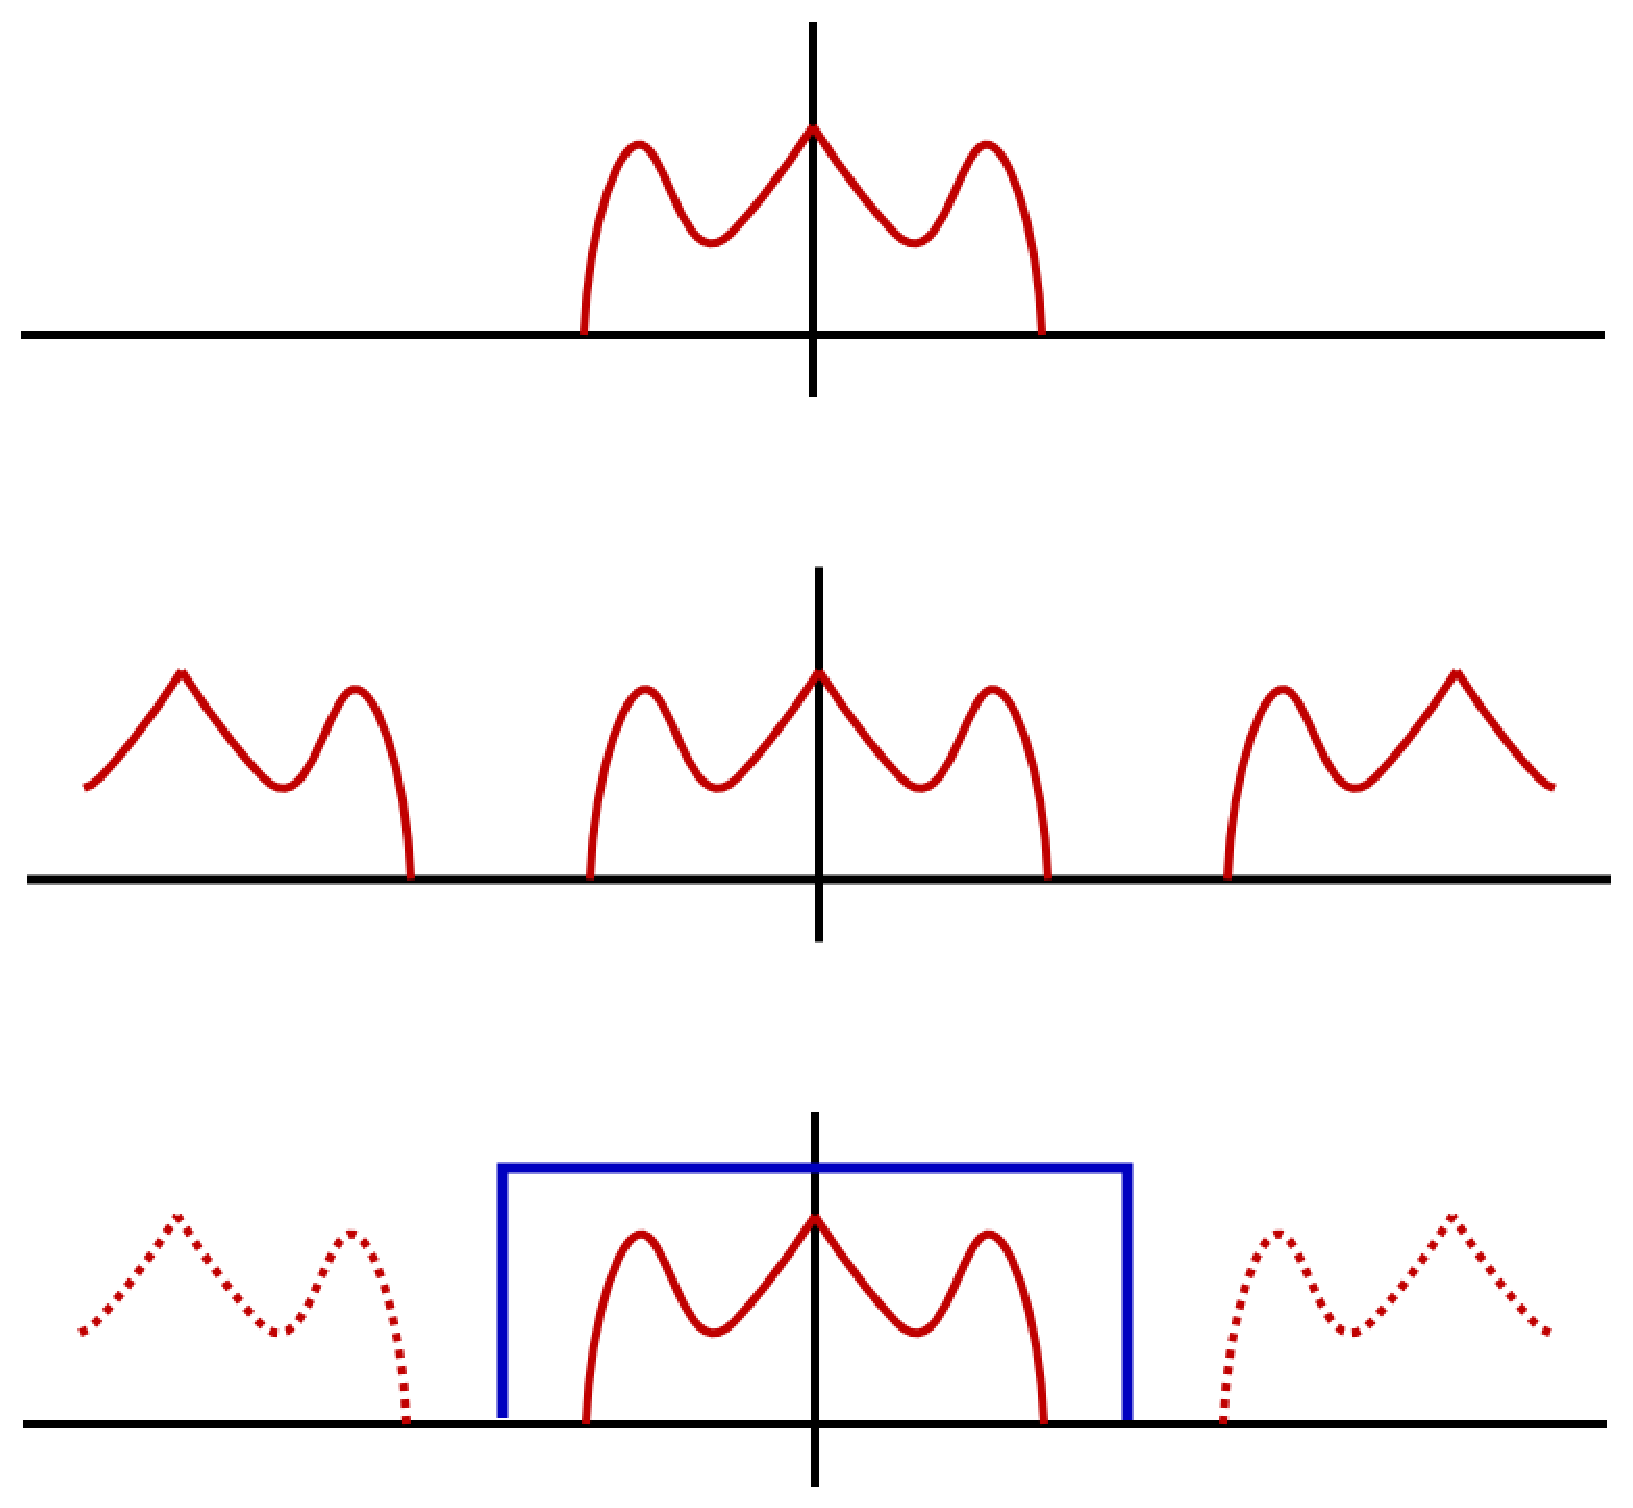
\epsfig{file=Figures/sampling,width=8cm}
\caption{The sampling and reconstruction of a bandwidth-limited signal.
When the sampling rate exceeds twice the bandwidth of the original signal, this signal can be reconstituted from its sampled values.}
\label{figure:Sampling}
\end{center}
\end{figure}
A succession of power spectral densities can be found on Figure~\ref{figure:Sampling}.
The top component shows the power spectral density of the original signal.
The density of the sampled signal appears below.
Finally, the reconstruction operation where a lowpass filter is employed to recovered the original function is illustrated at the bottom of the figure.
In contrast, Figure~\ref{figure:Aliasing} exhibits a case where the sampling frequency is too low.
\begin{figure}[thbp]
\begin{center}
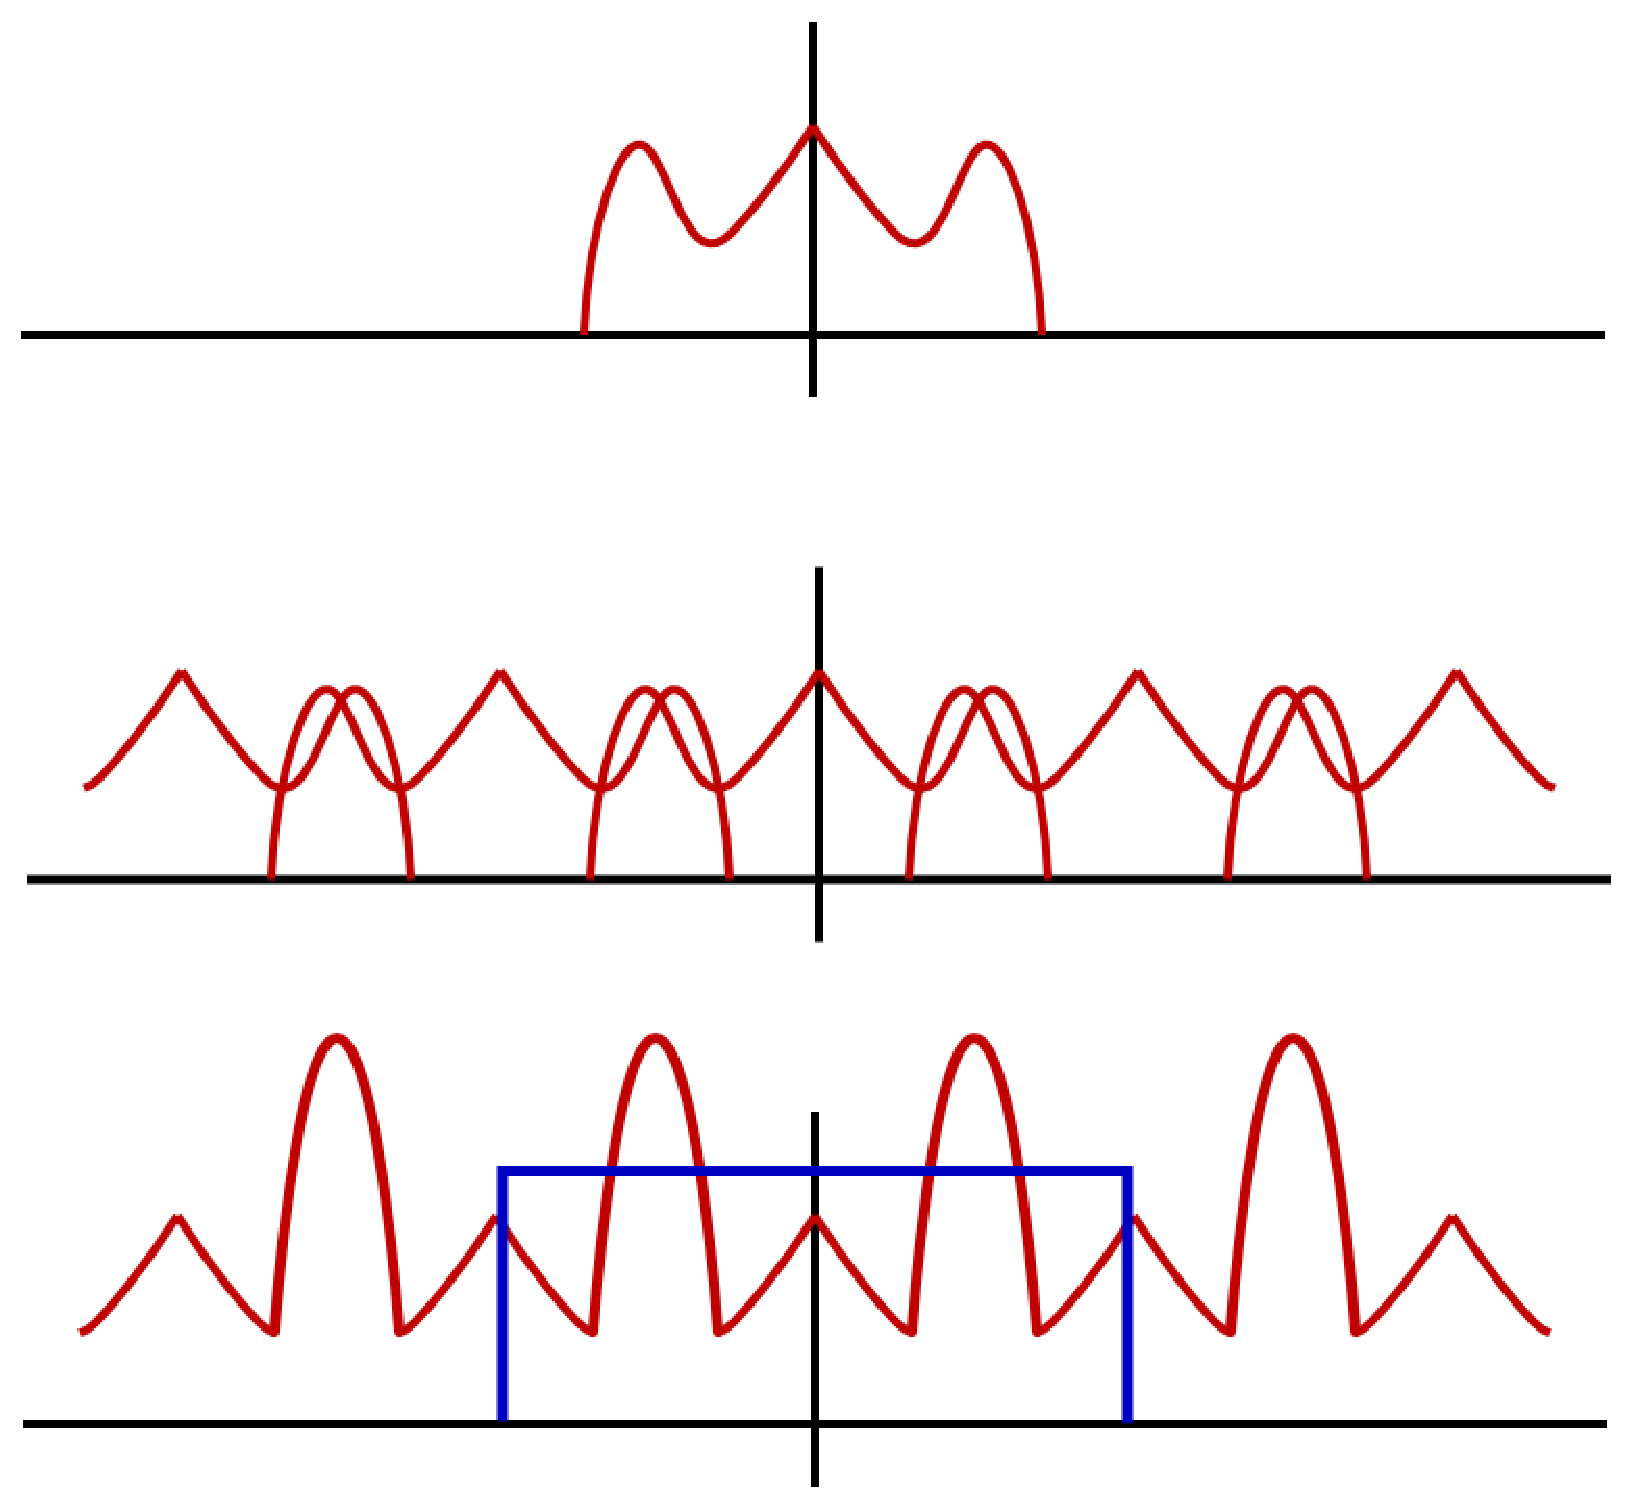
\epsfig{file=Figures/aliasing,width=8cm}
\caption{A low sampling frequency leads to aliasing, thereby preventing reconstruction of the original signal.}
\label{figure:Aliasing}
\end{center}
\end{figure}
Aliasing in the frequency domain prevents the original signal from being retrieved.

Sampling and aliasing are also important in film and video.
The illusion of a moving image in video is achieved by displaying a rapid succession of still pictures over time.
Films are typically shot at a rate of twenty-four frames per second, whereas the minimum frame rate required to create the appearance of a moving image is about fifteen frames per second.
The human eye acts as a lowpass filter and transforms the succession of images into a live video.
High-speed cameras are used to record slow-motion playback movies.
As a consequence, they must run at much higher frame-rates than normal cameras.

\subsection{The Sampling Theorem}

The sampling theorem is one of the most significant results in digital communication and signal processing.
Many digital communication systems rely on the validity of this theorem and on the design insights it provides for proper operation.

The basic idea behind the sampling theorem can be summarized in a few words.
If a signal $x(t)$ is bandwidth-limited to $W$, then this signal can be reconstructed from a collection of samples so long as the samples are taken at periodic intervals of $T \leq \frac{1}{2W}$.
A formal version of the sampling theorem appears below.

\begin{theorem}[Sampling Theorem] \label{theorem:SamplingTheorem}
Let signal $x(t)$ be a bandwidth-limited function with bandwidth $W$.
If $x(t)$ is sampled at times $\{ nT : n \in \mathbb{Z} \}$ where $T \leq \frac{1}{2W}$, then it is possible to reconstruct the original signal $x(t)$ from its sampled points $\{ x(nT) : n \in \mathbb{Z} \}$.
Specifically, if $T \leq \frac{1}{2W}$ then
\begin{equation} \label{equation:SamplingReconstructionFormula}
x(t) = \sum_{n = -\infty}^{\infty}
x(nT) \mathrm{sinc} \left( \frac{t}{T}-n \right) .
\end{equation}
\end{theorem}
\begin{proof}
The signal $x(t)$ is bandwidth-limited with bandwidth $W$.
It follows that $x(t)$ is the inverse Fourier transform of a function $\hat{x}(f)$, where $\hat{x}(f) = 0$ for all frequencies such that $|f| > W$.
For convenience, we define $F = \frac{1}{T}$ and we stress that $W \leq \frac{1}{2T} = \frac{F}{2}$.
Thus, $\hat{x}(f) = 0$ whenever $|f| > \frac{F}{2}$.
We can apply the theory of Fourier series introduced in Section~\ref{section:FourierSeries} to express $\hat{x}(f)$ as
\begin{equation*}
\hat{x}(f) = \sum_{k=-\infty}^{\infty} s_k e^{2 \pi i \frac{k}{F} f}
\mathrm{rect} \left( \frac{f}{F} \right)
\end{equation*}
where the coefficients $\{ s_k : k \in \mathbb{Z} \}$ are equal to
\begin{equation*}
s_k
= \frac{1}{F} \int_{-\frac{F}{2}}^{\frac{F}{2}}
\hat{x}(f) e^{- 2 \pi i \frac{k}{F} f} df .
\end{equation*}
Special care should be taken when reading these equations because we are applying Fourier series analysis to a function in the frequency domain.
This can get confusing.

We can then write $x(t)$ in terms of basis elements,
\begin{equation*}
\begin{split}
x(t) &= \mathcal{F}^{-1} \left[ \hat{x}(f) \right]
= \mathcal{F}^{-1} \left[ \sum_{k=-\infty}^{\infty} s_k e^{2 \pi i \frac{k}{F} f}
\mathrm{rect} \left( \frac{f}{F} \right) \right] \\
&= \sum_{k=-\infty}^{\infty} s_k \mathcal{F}^{-1} \left[ e^{2 \pi i \frac{k}{F} f}
\mathrm{rect} \left( \frac{f}{F} \right) \right] \\
%&= \sum_{k=-\infty}^{\infty} s_k
%\int_{-\frac{F}{2}}^{\frac{F}{2}} e^{2 \pi i \frac{k}{F} f} e^{2 \pi i f t} df \\
%&= \sum_{k=-\infty}^{\infty} s_k
%\int_{-\frac{F}{2}}^{\frac{F}{2}} e^{2 \pi i \left( t + \frac{k}{F} \right) f} df \\
%&= \sum_{k=-\infty}^{\infty} s_k
%\frac{e^{\pi i \left( t + \frac{k}{F} \right) F} - e^{-\pi i \left( t + \frac{k}{F} \right) F}}{2 \pi i \left( t + \frac{k}{F} \right)} \\
%&= \sum_{k=-\infty}^{\infty} s_k
%\frac{\sin \left( \pi \left( t + \frac{k}{F} \right) F \right)}{\pi \left( t + \frac{k}{F} \right)} \\
%&= \sum_{k=-\infty}^{\infty} s_k F \mathrm{sinc} \left( F t + k \right) \\
&= \sum_{k=-\infty}^{\infty} \frac{s_k}{T} \mathrm{sinc} \left( \frac{t}{T} + k \right) .
\end{split}
\end{equation*}
Above, we have successively used the scaling and time-shift properties of the Fourier transform.
We can obtain the values of $\{ s_k : k \in \mathbb{Z} \}$ explicitly by exploiting the characteristics of the $\mathrm{sinc} (\cdot)$ function,
\begin{equation*}
x(nT)
= \sum_{k=-\infty}^{\infty}
\frac{s_k}{T} \mathrm{sinc} \left( \frac{nT}{T} + k \right)
= \sum_{k=-\infty}^{\infty}
\frac{s_k}{T} \mathrm{sinc} ( n + k ) = \frac{s_{-n}}{T} .
\end{equation*}
Thus, we have $s_{k} = T x(-kT)$ and formula \eqref{equation:SamplingReconstructionFormula} follows.
The sampling rate $F = 2W$ associated with the sampling period $T = \frac{1}{2W}$ is the minimum rate at which perfect reconstruction is possible.
It is called the \defn{Fourier analysis}{Nyquist rate} in honor of Swedish-American engineer Harry Nyquist.
\end{proof}


\subsection{Imperfect Sampling and Reconstruction}

In practice, it is impossible to measure (i.e., sample) a signal $x(t)$ instantaneously.
A more realistic model is to assume that the sample value is obtained through the integral
\begin{equation*}
\int_{\mathbb{R}} x(t) p(t-nT) dt ,
\end{equation*}
for some sampling waveform $p(t)$.
In this case, the resulting samples are identical to the perfect sampling of the filtered waveform $u(t)=x(t)*p(-t)$.
That is, the sample values are given by
\begin{equation*}
u(nT) = \int_{\mathbb{R}} x(t) p(t-nT) dt .
\end{equation*}
It also follows that, if no aliasing occurs, the imperfection can be eliminated completely using a discrete-time filter to equalize the resulting samples.

A similar imperfection occurs during reconstruction.
In practice, it is not possible to weight each sample by the exact sinc interpolation waveform.
Instead, the samples $u(nT)$ are weighted by a pulse shape $q(t)$.
In this case, the reconstruction output is given by
\[ y(t) = \sum_{n=-\infty}^{\infty} u(nT) q(t-nT). \]
Since $q(t-nT) = \delta(t-nT) * q(t)$, we can see this instead as perfect reconstruction followed by filtering and write
\[ y(t) = \left( \sum_{n=-\infty}^{\infty} u(nT) \delta (t-nT) \right) * q(t) = u(t) * q(t). \]
Again, it follows that this imperfection can be eliminated completely by post-filtering.
In practice, the main advantage of this observation is that one can jointly optimize $p(t)$, $q(t)$ and the post-filter to provide good performance while using inexpensive components.


\newpage
\section{Stochastic Signals}
\label{section:StocahsticSignalsFAS}
\index{random process}

A \textbf{random process} (or \defn{random process}{stochastic process}) is an extension of the concept of random variable to the situation where the values of a signal are not known beforehand.
Mathematically, a stochastic process can be viewed in two different ways.
First, the process can be thought of as an instantiation of a random experiment where the outcome is selected from a collection of time functions.
Alternatively, a stochastic process can be viewed as a collection of random variables indexed by time.
If the index set corresponds to the real numbers, then the process is a \defn{random process}{continuous-time} \textbf{random process}.
Whereas if the index set is discrete, then it is a \defn{random process}{discrete-time} \textbf{random process}.
The viewpoint where a stochastic process is regarded as a collection of random variables tends to prevail in the study of digital communications.
\begin{figure}[htbp]
\begin{center}
\begin{psfrags}
\psfrag{A}[c]{Amplitude}
\psfrag{t}[c]{Time}
\psfrag{t0}[c]{$t_0$}
\psfrag{t1}[c]{$t_1$}
\epsfig{file=Figures/process,width=7cm}
\end{psfrags}
\caption{Two distinct abstractions of a random process.
It can be viewed as the output of an experiment where a function is selected at random.
Alternatively, a random process may be taken as a set of random variables indexed by time.}
\label{figure:RandomProcess}
\end{center}
\end{figure}

Random processes are frequently employed in the design of communication systems.
For example, they can be used to model the data originating from a source, channel variations, noise and interference.
Their importance will become evident as we progress through these notes.
In general, it is difficult to provide a complete mathematical description for a random process.
For now, we restrict our attention to \defn{random process}{stationary} and \defn{random process}{ergodic} random processes.

\begin{definition}[Stationarity]
A random process $X(t)$ is wide-sense stationary (WSS) if its \defn{random process}{mean}
\begin{equation*}
m_X(t) \triangleq \mathrm{E} [X(t)]
\end{equation*}
is independent of time, and its \defn{random process}{autocorrelation function}, defined by
\begin{equation*}
R_X(t_1, t_2) \triangleq \mathrm{E} [X(t_1) X^*(t_2)],
\end{equation*}
only depends on the difference between $t_1$ and $t_2$.
With a slight abuse of notation, we can denote the mean and autocorrelation of a stationary process respectively by $m_X$ and $R_X(\tau)$, where $\tau = t_1 - t_2$.
\end{definition}

\begin{figure}[htbp]
\begin{center}
\begin{psfrags}
\psfrag{A}[c]{Amplitude}
\psfrag{t}[c]{Time}
\psfrag{t0}[c]{$t_0$}
\psfrag{m}[c]{$m_X$}
\psfrag{e}[c]{$\lim_{T \rightarrow \infty} \frac{1}{T} \int_{- \frac{T}{2}}^{\frac{T}{2}} X(t) dt$}
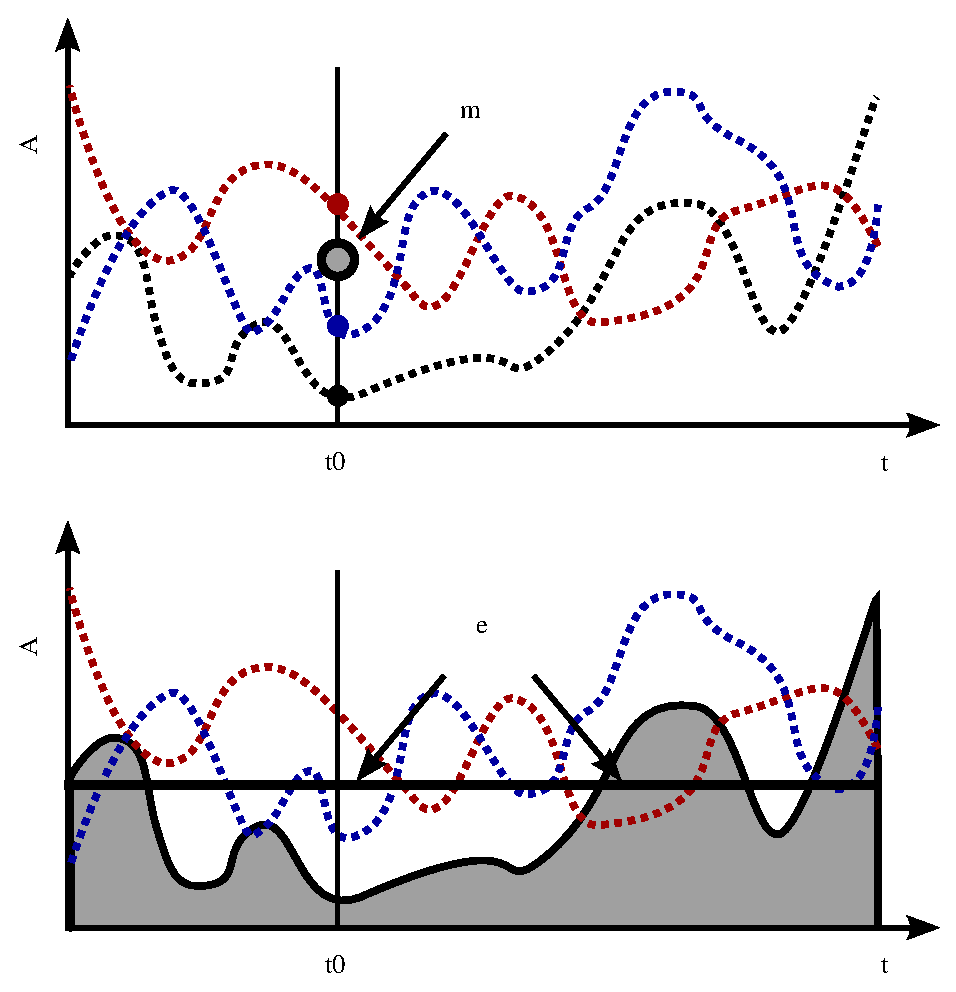
\epsfig{file=Figures/ergodic,width=8cm}
\end{psfrags}
\caption{For ergodic processes, the time average of a function along a trajectory is equal to the ensemble average.}
\label{figure:ErgodicProcess}
\end{center}
\end{figure}

\begin{definition}[Ergodic]
An \textbf{ergodic theorem} asserts that, under certain conditions, the time average of a random process
\begin{equation*}
\langle g(X(t)) \rangle \triangleq \lim_{T \rightarrow \infty} \frac{1}{T} \int_{- \frac{T}{2}}^{\frac{T}{2}} g(X(t)) dt
\end{equation*}
exists and is equal to the ensemble average $\mathrm{E}[g(X(t))]$ for almost all trajectories of the random process.
% exists and is equal to its ensemble average,
%\begin{equation*}
%\langle g(X(t)) \rangle \triangleq \lim_{T \rightarrow \infty} \frac{1}{T} \int_{- \frac{T}{2}}^{\frac{T}{2}} g(X(t)) dt
%= \mathrm{E}[g(X(t))] .
%\end{equation*}
When a stochastic process fulfills these conditions, it is called \defn{random process}{ergodic}.
\end{definition}

One of the important characteristics of an ergodic process is that it suffices to look at one realization of the process to infer many of its statistical attributes.
Ergodicity is a very strong property, and it is hard to test and validate.
Rather, it is frequently taken as a premise in the design of communication systems.
For instance, most information sources are assumed to be stationary and ergodic.
Such a postulate appears reasonable, especially considering the many successful communication systems implemented based on this assumption.


\subsection{Power Spectral Density}

For a stochastic signal, the definition of the \defn{random process}{power spectral density} is somewhat more intricate because it must account for uncertainty in the process.
Let $X(t)$ be a wide-sense stationary random process with $R_X(0) < \infty$.
Then, we can define
\begin{equation*}
\hat{X}_T(f) \triangleq \mathcal{F} \left[ X(t) \mathrm{rect} \left( \frac{t}{T} \right) \right] 
\end{equation*}
and
\begin{equation*}
\mathcal{S}_X(f) \triangleq \lim_{T \rightarrow \infty} \frac{1}{T} \mathrm{E} \left[ |\hat{X}_T(f)|^2 \right] .
\end{equation*}

As we will soon see, the power spectral density plays an instrumental role in the sampling theorem for random signals.
First, we provide a means to compute $\mathcal{S}_X(f)$ from its statistical attributes.

\begin{theorem}[Wiener-Khinchin] \label{theorem:WienerKhinchin}
The power spectral density $\mathcal{S}_X (f)$ of a wide-sense stationary random process $X(t)$ is equal to the Fourier transform of its autocorrelation function, $\mathcal{S}_X (f) = \mathcal{F} [R_X (\tau)]$.
\end{theorem}
\begin{proof}
For a wide-sense stationary process, we have
\begin{equation*}
\begin{split}
\mathcal{S}_X(f) &= \lim_{T \rightarrow \infty} \frac{1}{T} \mathrm{E} \left[ |\hat{X}_T(f)|^2 \right]
= \lim_{T \rightarrow \infty} \frac{1}{T} \mathrm{E} \left[ \hat{X}_T(f) \hat{X}_T^*(f) \right] \\
&= \lim_{T \rightarrow \infty} \frac{1}{T} \mathrm{E} \left[
\int_{-\frac{T}{2}}^{\frac{T}{2}} X(t_1) e^{-2 \pi i f t_1} dt_1
\int_{-\frac{T}{2}}^{\frac{T}{2}} X^*(t_2) e^{2 \pi i f t_2} dt_2 \right] \\
&= \lim_{T \rightarrow \infty} \frac{1}{T}
\int_{-\frac{T}{2}}^{\frac{T}{2}} \int_{-\frac{T}{2}}^{\frac{T}{2}}
\mathrm{E} \left[ X(t_1) X^*(t_2) \right]
e^{-2 \pi i f (t_1-t_2)} dt_1 dt_2 \\
&= \int_{\mathbb{R}} R_X (\tau) e^{-2 \pi i f\tau} d\tau
= \mathcal{F} [ R_X (\tau) ] .
\end{split}
\end{equation*}
The fourth equality is obtained by interchanging the expectation and the integrals, while the sixth equality follows from a change of variables and the fact that $X(t)$ is wide-sense stationary.
To guarantee that the former operation is legitimate, $\tau R_X(\tau)$ must remain finite for all $\tau$.
\end{proof}

In some cases, it may be possible to estimate the power spectral density from a single realization of $X(t)$.
For example, the autocorrelation of $X(t)$ is ergodic if it satisfies
\begin{equation*}
\langle X(t) X^* (t-\tau) \rangle \triangleq \lim_{T \rightarrow \infty} \frac{1}{T} \int_{- \frac{T}{2}}^{\frac{T}{2}} X(t) X^* (t-\tau) dt = \mathrm{E} \left[ X(t) X^*(t-\tau) \right].
\end{equation*}
In this case, the expectation in the theorem above can be replaced by a time average and the result can be computed from a single realization.

\subsection{Filtering Stochastic Processes}

We discussed in Section~\ref{subsection:LinearTimeInvariantFilters} how the Fourier transform can simplify the analysis of the effects of linear time-invariant filters on deterministic signals.
In this section, we consider the operation of such filters in the context of random processes.

\begin{theorem} \label{theorem:filteredWSS}
If a wide-sense stationary process $X(t)$ with mean $m_X$ and autocorrelation function $R_X(\tau)$ is passed through a linear time-invariant filter with impulse response $h(t)$, then the output process $Y(t)$ has mean
\begin{equation*}
m_Y = m_X \int_{\mathbb{R}} h(t) dt
\end{equation*}
and its autocorrelation is equal to
\begin{equation*}
R_Y (\tau) = R_X(\tau) \ast h(\tau) \ast h^*(-\tau) .
\end{equation*}
\end{theorem}
\begin{proof}
The output process at time~$t$ is given by $Y(t) = \int_{\mathbb{R}} X(t - \xi) h(\xi) d\xi$.
We can therefore obtain the expectation of $Y(t)$ as follows,
\begin{equation*}
\begin{split}
m_Y (t) &= \mathrm{E} \left[ \int_{\mathbb{R}} X(t - \xi) h(\xi) d\xi \right]
= \int_{\mathbb{R}} \mathrm{E} \left[ X(t - \xi) \right] h(\xi) d\xi \\
&= m_X \int_{\mathbb{R}} h(\xi) d\xi.
\end{split}
\end{equation*}
We emphasize that $m_Y$ is independent of time.

To derive the autocorrelation function for $Y(t)$, we first compute the cross-correlation between $X(t)$ and $Y(t)$,
\begin{equation} \label{equation:CrossCorrelationLTI}
\begin{split}
\mathrm{E} [X(t_1) Y^*(t_2) ]
&= \mathrm{E} \left[ X(t_1) \int_{\mathbb{R}} X^*(\xi) h^*(t_2 - \xi) d\xi \right] \\
&= \int_{\mathbb{R}} \mathrm{E} \left[ X(t_1) X^*(\xi) \right] h^*(t_2 - \xi) d\xi \\
&= \int_{\mathbb{R}} R_X(t_1 - \xi) h^*(t_2 - \xi) d\xi \\
%&= \int_{\mathbb{R}} R_X(\tau - \xi) h^*(- \xi) d\xi \\
&= R_X(\tau) \ast h^*(-\tau) .
\end{split}
\end{equation}
This shows that the cross-correlation between $X(t)$ and $Y(t)$ depends only on $\tau$; we can therefore express it as $R_{XY}(\tau)$.
We are now ready to compute the autocorrelation function for $Y(t)$.
\begin{equation} \label{equation:AutoCorrelationLTI}
\begin{split}
\mathrm{E} [Y(t_1) Y^*(t_2) ]
&= \mathrm{E} \left[ \int_{\mathbb{R}} X(\xi) h(t_1 - \xi) d\xi Y^*(t_2) \right] \\
&= \int_{\mathbb{R}} \mathrm{E} \left[ X(\xi) Y^*(t_2) \right] h(t_1 - \xi) d\xi \\
&= \int_{\mathbb{R}} R_{XY}(\xi - t_2) h(t_1 - \xi) d\xi \\
%&= \int_{\mathbb{R}} R_{XY}(\xi) h(\tau - \xi) d\xi \\
&= R_{XY}(\tau) \ast h(\tau) .
\end{split}
\end{equation}
Substituting $R_{XY} (\tau)$ by the equivalent expression $R_X(\tau) \ast h^*(-\tau)$ from \eqref{equation:CrossCorrelationLTI}, we get the desired result.
We observe that the autocorrelation of the process $Y(t)$ only depends on the difference between $t_1$ and $t_2$, and hence $Y(t)$ is also wide-sense stationary.
\end{proof}

Obtaining an expression for the autocorrelation function corresponding to the output of a linear time-invariant filter allows us to characterize the power spectral density of the output process.
In terms of the frequency representation, we get $m_Y = m_X \hat{h}(0)$ and
\begin{equation*}
\begin{split}
\mathcal{S}_Y (f) &= \mathcal{F} [ R_Y (\tau) ] \\
&= \mathcal{F} \left[ R_X (\tau) \ast h(\tau) \ast h^*(-\tau) \right] \\
&= \mathcal{S}_X(f) | \hat{h}(f) |^2 .
\end{split}
\end{equation*}
A linear time-invariant filter can be employed to shape the spectrum of a stochastic process, and to constrain its bandwidth.
This is an important result, as linear filters can be used to reduce the bandwidth of a random signal before sampling or to reconstruct a random signal from its samples.

\subsection{Gaussian Processes}

A stochastic process $X(t)$ is a \defn{random process}{Gaussian process} if, for any finite set of sampling times $t_1, t_2, \ldots, t_n$, the resulting random variables $X(t_1),X(t_2),\ldots,X(t_n)$ are jointly Gaussian random variables.
The distribution of jointly Gaussian random variables is completely determined by their mean vector and correlation matrix.
Therefore, a Gaussian process is completely determined by its mean function $m_X (t)$ and its autocorrelation function $R_XX (t_1,t_2)$.
Of course, if the process is also wide-sense stationary, then this reduces to its mean value $m_X$ and its autocorrelation function $R_X (\tau)$.

More generally, one finds that, for any finite set of energy-type signals $s_1 (t), s_2 (t), \ldots , s_n (t)$, the random variables
\[ Z_i = \int_{-\infty}^{\infty} s(t) X(t) dt \]
are jointly Gaussian.
The intuition behind this is that each integral is defined as the limit of a sequence of Riemann sums.
Since each Riemann sum is simply the sum of Gaussian random variables, it is also Gaussian.
This argument can be extended to show that the mean vector and correlation matrix of the vector $(Z_1, Z_2, \ldots, Z_n)$ is also jointly Gaussian.
In fact, combining this with Theorem~\ref{theorem:filteredWSS}, implies that the output of linear time-invariant system, whose input is a wide-sense stationary Gaussian process, is also a wide-sense stationary Gaussian process. 

The most common random process in signal processing and communications is the \defn{random process}{Gaussian white-noise} process $N(t)$.
This process is defined to be a zero-mean wide-sense stationary Gaussian process whose power spectral density $S_N (f)$ is constant (e.g., 1).
Since this process has infinite power, it is not particularly well-defined mathematically.
Still, we can use the cavalier Fourier transform $\mathcal{F} [ 1 ] = \delta(t)$ to argue that the autocorrelation function of $N(t)$ should be $R_N (\tau) = \delta(\tau)$.
In practice, this is not a problem because $N(t)$ is only used as the input to a linear filter whose output process is guaranteed to have finite power.

\section{Sampling Bandlimited Processes}

We know from Theorem~\ref{theorem:SamplingTheorem} that a bandwidth-limited signal can be perfectly reconstructed from its samples provided that the sampling rate exceeds twice the bandwidth of the original signal.
At this point, one may wonder whether it is possible to extend the sampling theorem to bandwidth-limited stochastic processes.
This question is answered in the affirmative below.

\begin{theorem} \label{theorem:SamplingRandomSignals}
Suppose that $X(t)$ is a wide-sense stationary bandwidth-limited process with bandwidth $W$ and power spectral density $\mathcal{S}_X (f)$.
Let $\tilde{X}(t)$ be an approximation for $X(t)$ built from the sampled values $\{ X(nT) : n \in \mathbb{Z} \}$,
\begin{equation*}
\tilde{X}(t) = \sum_{n=-\infty}^{\infty} X(nT) \mathrm{sinc} (2 W (t - nT)) ,
\end{equation*}
where $T = \frac{1}{2W}$ denotes the sampling interval.
Then the mean-squared error between the original random process and the reconstructed version vanishes,
\begin{equation} \label{equation:SamplingMSE}
\left\| X(t) - \tilde{X}(t) \right\|^2
= \mathrm{E} \left[ \left| X(t) - \sum_{n=-\infty}^{\infty}
X(nT) \mathrm{sinc} (2 W (t - nT)) \right|^2 \right] = 0 .
\end{equation}
The expectation in \eqref{equation:SamplingMSE} is over all possible realizations of $X(t)$.
\end{theorem}
\begin{proof}
To establish this result, we expand the mean-squared error of \eqref{equation:SamplingMSE},
\begin{equation*}
\begin{split}
&\left\| X(t) - \tilde{X}(t) \right\|^2
= \mathrm{E} \left[ \left| X(t) - \sum_{n=-\infty}^{\infty} X(nT)
\mathrm{sinc}(2 W (t - nT)) \right|^2 \right] \\
&= R_X(0) - \sum_{n=-\infty}^{\infty} [ R_X(t-nT) + R_X^*(t-nT) ]
\mathrm{sinc}(2 W (t - nT)) \\
&+ \sum_{n=-\infty}^{\infty} \sum_{m=-\infty}^{\infty} R_X((m-n)T)
\mathrm{sinc}(2 W (t - mT)) \mathrm{sinc}(2 W (t - nT)) .
\end{split}
\end{equation*}
The double summation above can be rewritten as
\begin{equation*}
\begin{split}
&\sum_{n=-\infty}^{\infty} \sum_{k=-\infty}^{\infty} R_X(kT)
\mathrm{sinc}(2 W (t - kT - nT)) \mathrm{sinc}(2 W (t - nT)) \\
&\sum_{n=-\infty}^{\infty} \left( \sum_{k=-\infty}^{\infty} R_X(kT)
\mathrm{sinc}(2 W (t - kT - nT)) \right) \mathrm{sinc}(2 W (t - nT)) \\
&= \sum_{n=-\infty}^{\infty} R_X(t - nT) \mathrm{sinc}(2 W (t - nT)) ,
\end{split}
\end{equation*}
where the last equality follows from the sampling theorem for deterministic signals (Theorem~\ref{theorem:SamplingTheorem}).
Putting these results together, we get
\begin{equation*}
\left\| X(t) - \tilde{X}(t) \right\|^2
= R_X(0) - \sum_{n=-\infty}^{\infty} R_X^*(t-nT) \mathrm{sinc}(2 W (t - nT)) .
\end{equation*}
Applying Theorem~\ref{theorem:SamplingTheorem} one more time and noticing that $R_X(0) = R_X^*(0)$, we obtain $\| X(t) - \tilde{X}(t) \|^2 = 0$, as desired.
\end{proof}

Theorem~\ref{theorem:SamplingRandomSignals} is important because it confirms that the design insights gained from analyzing deterministic signals hold for random signals as well.


\section{Bandpass Signals and Processes}

One possible application of sampling is to take a continuous-time signal and to transform it into a discrete-time signal.
For instance, this operation gives the information coming out of a source a format more suitable for digital communications.
This prime application of sampling served as the original motivation for our study of the subject.
A second possible application of sampling is the processing of received waveforms at the output of communication channels.
In digital communications, the data often assumes the form of an analog carrier signal modulated by a digital bit stream.
Mathematically, this situation is captured by the equation
\begin{equation*}
y(t) = x(t) \cos (2 \pi f_{\mathrm{c}} t) .
\end{equation*}
The signal $y(t)$ is a special form of a \defn{Fourier analysis}{bandpass signal}.
Its Fourier transform $\hat{y}(f)$ is non-zero only for frequencies contained in a small neighborhood of carrier frequency $f_{\mathrm{c}}$.
That is, $\hat{y}(f) = 0$ for all frequencies such that $|f - f_{\mathrm{c}}| \geq W$.
To apply the sampling tools derived above to the information bearing signal $x(t)$, we need to shift the corresponding spectrum to the origin.

The Fourier transform of $y(t)$ is given by
\begin{equation*}
\hat{y}(f) = \frac{1}{2} \hat{x}(f+f_{\mathrm{c}}) + \frac{1}{2} \hat{x}(f - f_{\mathrm{c}}) .
\end{equation*}
Our strategy is to first eliminate $\frac{1}{2} \hat{x}(f + f_{\mathrm{c}})$ from $\hat{y}(f)$, and then to scale and shift $\frac{1}{2} \hat{x}(f + f_{\mathrm{c}})$ back to the origin.
Define the \defn{Fourier analysis}{step function} by
\begin{equation*}
\mathrm{step} (t) = \frac{1}{2} + \frac{1}{2} \mathrm{sign}(t). 
\end{equation*}
Taking the (cavalier) Fourier transform of $\mathrm{step}(t)$, we get
\begin{equation*}
\begin{split}
{\mathcal{F}} [\mathrm{step} (t)]
&= {\mathcal{F}} \left[ \frac{1}{2} + \frac{1}{2} \mathrm{sign}(t) \right] \\
&= \frac{1}{2} \delta (f)
- \frac{1}{2} \int_{-\infty}^0 e^{-2 \pi i ft} dt
+ \frac{1}{2} \int_0^{\infty} e^{-2 \pi i ft} dt \\
&= \frac{1}{2} \delta(f)  + \frac{1}{2 \pi i f}.
\end{split}
\end{equation*}
Using the duality property of the Fourier transform, we get
\begin{equation*}
\mathcal{F}^{-1} [\mathrm{step}(f)] = \frac{1}{2} \delta(t) + \frac{i}{2 \pi t} .
\end{equation*}
And, by construction, we obtain $\hat{x}(f - f_{\mathrm{c}}) = 2 \mathrm{step}(f) \hat{y}(f)$.
We can therefore recover the original lowpass signal $x(t)$ using the frequency-shift property of the Fourier transform,
\begin{equation*}
x(t)
= \left[ y(t) \ast \left( \delta (t) + \frac{i}{\pi t} \right) \right]
e^{- 2 \pi i f_{\mathrm{c}} t}
= \left[ y(t) + i \left( y(t) \ast \frac{1}{\pi t} \right) \right] e^{- 2 \pi i f_{\mathrm{c}} t} .
\end{equation*}
The second component of this signal,
\begin{equation*}
y(t) \ast \frac{1}{\pi t} ,
\end{equation*}
is called the \defn{Fourier analysis}{Hilbert transform} of $y(t)$.
Once $x(t)$ is brought back to baseband, the standard sampling theorem applies and a discrete-time version of the signal can be produced.

% Bandpass processes
